\section{Descripción del modelo del circuito}

\subsection{Circuito de Chua}

\begin{frame}
	\frametitle{\subsecname}

	\begin{itemize}
		\item

		      \eqref{eq:chua}~es un sistema EDO no lineal autónomo.
		      Comprobado experimentalmente en~\citeyear{Zhong:M84/56}
		      por~\Citeauthor{Zhong:M84/56}.

		      \


		\item

		      Considere el circuito de la Figura~\ref{fig:chua_circuit}
		      con una \alert{resistencia no lineal $N_{R}$} de tres
		      segmentos lineal por tramos.

		      \

		\item

		      En el trabajo~\Citetitle{1085459} estudiamos el
		      comportamiento caótico del circuito y un
		      \alert{método de convergencia de órbitas} que nos ayudará
		      a estabilizar el mismo.
	\end{itemize}

	\

	\begin{minipage}{0.55\textwidth}
		\begin{equation}\label{eq:chua}
			\left.
			\begin{aligned}
				\diff{V_{C_{1}}}{t} & =\frac{1}{RC_{1}}(V_{C_{2}} - V_{C_{1}} - g(V_{C_{1}})) \\
				\diff{V_{C_{2}}}{t} & =\frac{1}{RC_{2}}(V_{C_{1}} - V_{C_{2}} + Ri_{L})       \\
				\diff{i_{L}}{t}     & =-\frac{1}{L}V_{C_{2}}
			\end{aligned}
			\right\}
			\text{\alert{Sistema de Chua}}
		\end{equation}
		donde
		\begin{itemize}
			\item

			      $V_{C_{1}}$, $V_{C_{2}}$ son los voltajes en los capacitores $C_{1}$, $C_{2}$, y

			\item

			      $g\left(V_{C_{1}}\right)$ es la \alert{curva característica} del \emph{diodo de Chua}.
		\end{itemize}
	\end{minipage}
	\begin{minipage}{0.35\textwidth}
		\begin{figure}[ht!]
			\centering
			\includesvg[width=0.35\paperwidth]{chua_circuit}
			\caption{
				Circuito de Chua conformado por la resistencia lineal $R$,
				inductancia lineal $L$ e $i_{L}$ es la intensidad de corriente.
			}\label{fig:chua_circuit}
		\end{figure}
	\end{minipage}

\end{frame}
\note{
	El término diodo de Chua es una descripción general de una resistencia no lineal de dos terminales
	con curva característica lineal por tramos.

	El diode de Chua no es único.
}

\subsection{Sistema de Chua adimensional}

\begin{frame}
	\frametitle{\subsecname}
	\begin{minipage}{0.55\textwidth}
		\begin{equation}\label{eq:chua_adimensional}
			\left\{
			\begin{aligned}
				\diff{x}{t} & = \alpha\left(y - x - g\left(x\right)\right) \\
				\diff{y}{t} & = x - y + z                                  \\
				\diff{z}{t} & = -\beta y
			\end{aligned}
			\right.
		\end{equation}
		y cuyos puntos de equilibrio son
		\begin{align*}
			P^{+} & =\left(1,0,-1\right) \\
			O     & =\left(0,0,0\right)  \\
			P^{-} & =\left(-1,0,1\right) \\
		\end{align*}
	\end{minipage}
	\begin{minipage}{0.35\textwidth}
		\begin{figure}[ht!]
			\centering
			\includesvg[width=0.35\paperwidth]{characteristic_curve}
			\caption{
				Curva caracterísitica de la resistencia no lineal $g\left(x\right)$ definida como
			}\label{fig:piecewise} % Intensidad de corriente versus voltaje.
		\end{figure}
		\begin{equation*}
			g\left(x\right)=
			\begin{cases}
				m_{0}x + m_{0} + m_{1} & \text{si } x\leq -1,   \\
				m_{1}x                 & \text{si } -1 < x < 1, \\
				m_{0}x + m_{1} - m_{0} & \text{si } x \geq 1.
			\end{cases}
		\end{equation*}
	\end{minipage}
\end{frame}
\note{
	Es antisimétrica, osea $\left(x,y,z\right)\to\left(-x,-y,z\right)$ no cambia la ecuación.

	\begin{equation*}
		\frac{\mathrm{d} x}{\mathrm{~d} t}=P x+q \psi\left(r^{*} x\right) \quad, x \in R^{3}
	\end{equation*}
	donde
	\begin{math}
		P=
		\left(\begin{array}{ccc}
			-a(1+m) & a  & 0  \\
			1       & -1 & 1  \\
			0       & -b & -c
		\end{array}\right),
		q=
		\left(\begin{array}{c}
			-a \\ 0 \\ 0
		\end{array}\right),
		r=
		\left(\begin{array}{l}
			1 \\ 0 \\ 0
		\end{array}\right),
	\end{math}
	y $\psi(\sigma)=0.5(n-m)(|\sigma+1|-|\sigma-1|)$
}

\section{Método para determinar el caos}

\subsection{Mapa de Poincaré}

\begin{frame}
	\frametitle{\subsecname~\parencite[Sección 5.3, pág. 168]{Viana2021}}

	\begin{minipage}{0.6\textwidth}
		\begin{definition}{Mapa de Poincaré}{poincaremap}
			Es la aplicación que asocia los puntos en $V\subset\Sigma$ abierto
			tal que las trayectorias que inician en $V$ retornan a $\Sigma$
			\begin{align*}
				P\colon V & \to\Sigma                                      \\
				x         & \mapsto\phi\left(\tau\left(x\right), x\right),
			\end{align*}
			donde $\tau\left(x\right)$ es el primer retorno del punto $x$ a
			$\Sigma$.

			Además, decimos que $\Sigma$ es la sección transversal al campo
			vectorial $\diff{x}{t}=f\left(x\right)$, $x\left(t_{0}\right)=x_{0}$.
		\end{definition}
	\end{minipage}
	\begin{minipage}{0.3\textwidth}
		\begin{figure}[ht!]
			\centering
			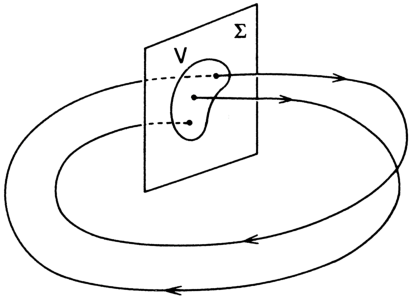
\includegraphics[width=0.35\paperwidth]{poincaremap}
			% \caption{Mapa de Poincaré para una órbita periódica.}\label{fig:poincaremap}
		\end{figure}
	\end{minipage}

\end{frame}

\note{
	$V\subset\Sigma$ abierto (por el teorema de existencia y unicidad para un campo vectorial $f$ de clase $C^{r}$)
}

\subsection{Exponentes de Lyapunov}

\begin{frame}
	\frametitle{\subsecname}

	\begin{figure}[ht!]
		\centering
		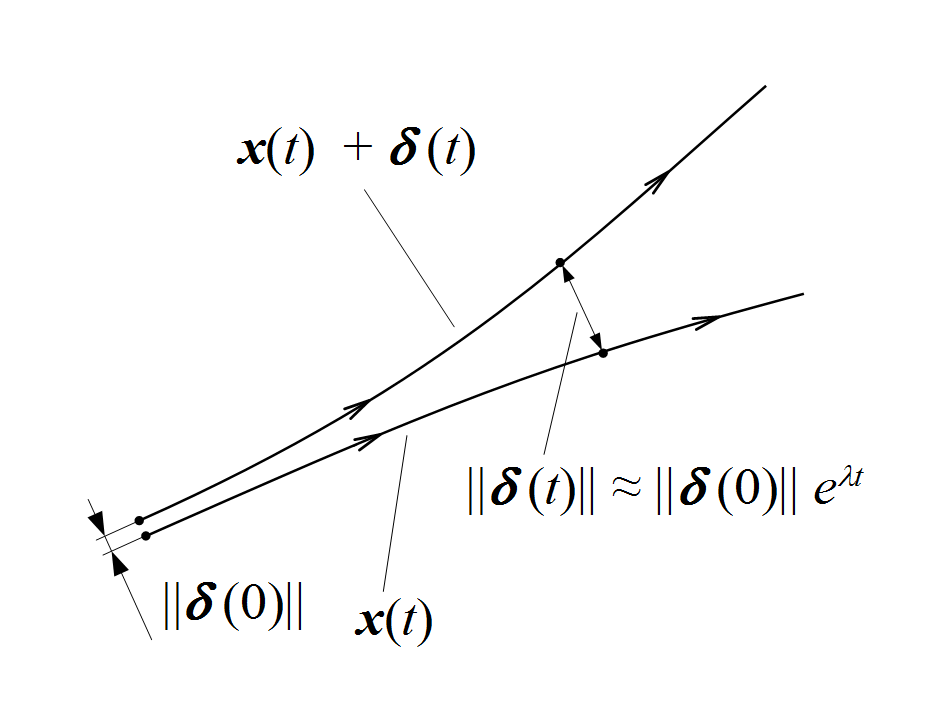
\includegraphics[width=0.7\paperwidth]{lyapunov}
	\end{figure}
\end{frame}

\section{Simulaciones numéricas}

\begin{frame}
	\frametitle{\secname~$\left(\alpha=10.0, \beta=16.4, m_{0}=-1.22, m_{1}=0.628\right)$}

	\begin{minipage}{0.45\textwidth}
		\begin{figure}[ht!]
			\centering
			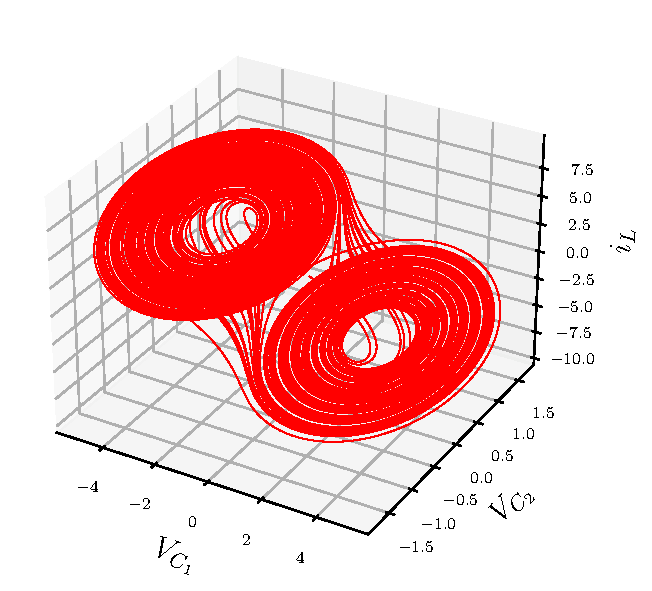
\includegraphics[width=0.45\paperwidth]{chua_double_scroll}
			\caption{
				Sistema dinámico del doble atractor de Chua.
			}\label{fig:chua_double_scroll}
		\end{figure}
	\end{minipage}
	\begin{minipage}{0.45\textwidth}
		\begin{figure}[ht!]
			\centering
			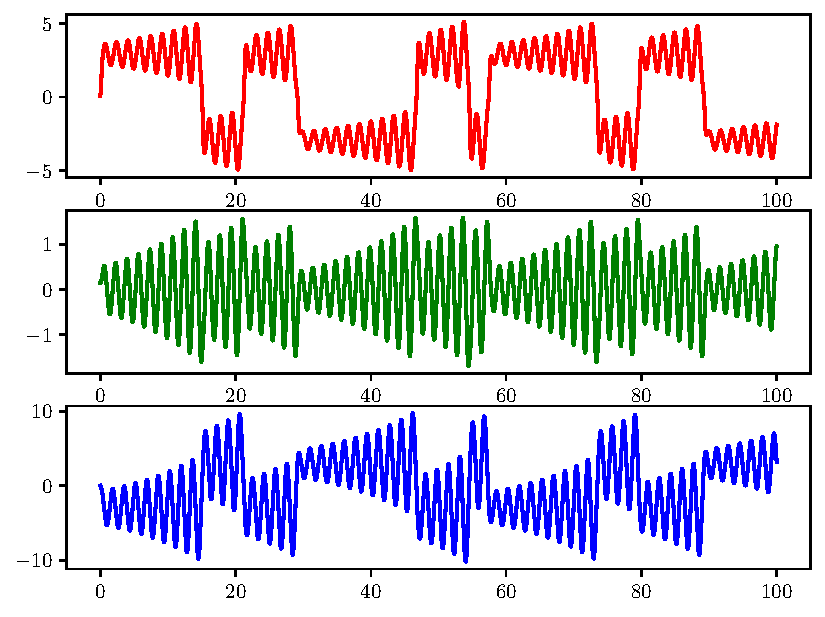
\includegraphics[width=0.45\paperwidth]{chua_solutions}
			\caption{
				Serie de tiempo.
			}\label{fig:chua_solutions}
		\end{figure}
	\end{minipage}
\end{frame}

\begin{frame}
	\frametitle{\secname} % \quad$\left(\beta_{1}=16.4,\beta_{2}=16.401\right)$

	\begin{figure}[ht!]
		\centering
		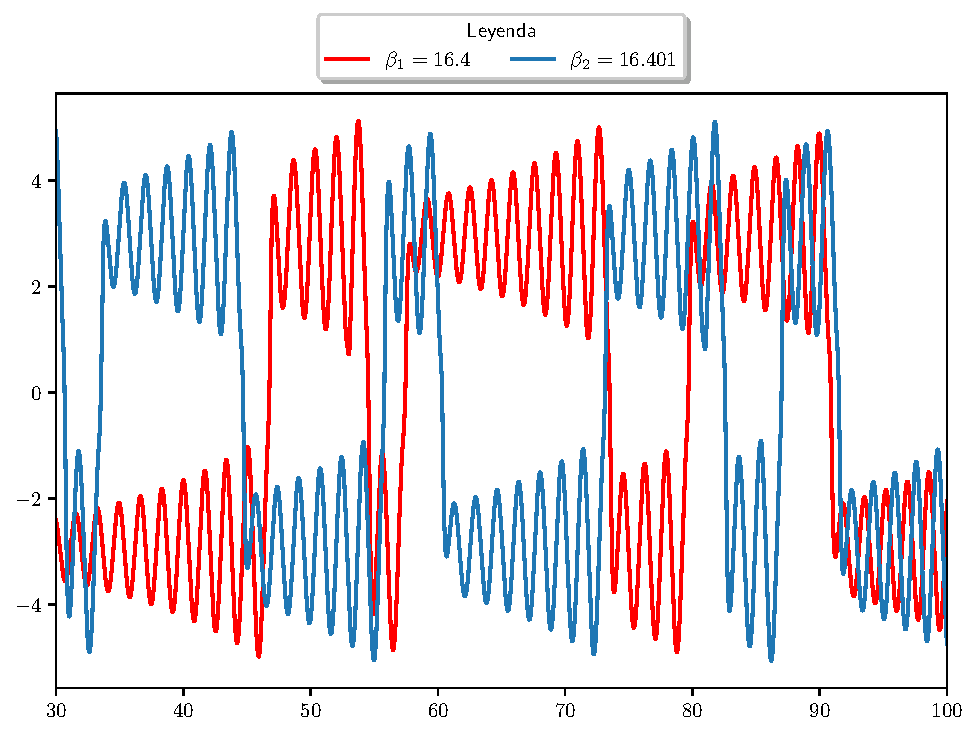
\includegraphics[width=0.58\paperwidth]{changing_beta}
		\caption{
			Soluciones de $V_{C_{1}}$ cuando $\beta_{1}\approx\beta_{2}$ y los demás parámetros constantes.
		}\label{fig:changing_beta}
	\end{figure}

\end{frame}

\begin{frame}
	\frametitle{\secname\quad$\left(\alpha=10,\beta=16.4,m_{0}=-1.22,m_{1}=0.728\right)$}

	\begin{minipage}{0.45\textwidth}
		\begin{figure}[ht!]
			\centering
			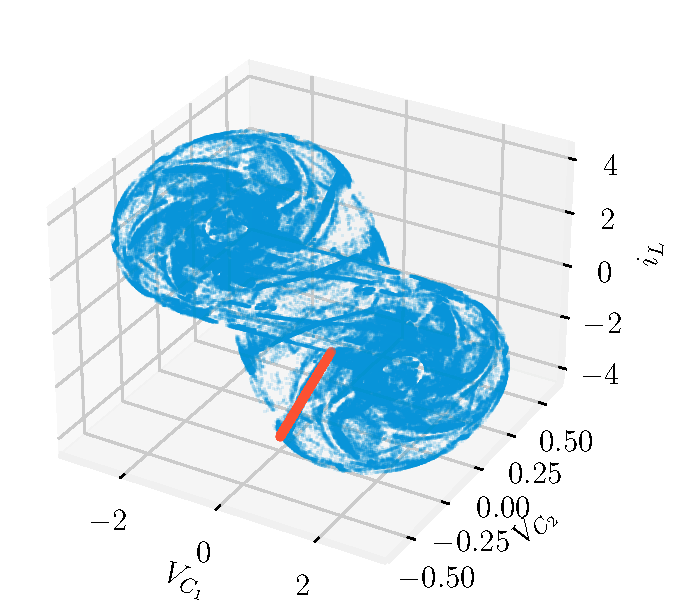
\includegraphics[width=0.44\paperwidth]{chua_double_atractor}
			\caption{
				La sección transversal es el plano
				\begin{math}
					\Sigma=\left\{\left(V_{C_{1}},V_{C_{2}},i_{L}\right):V_{C_{1}}=1\right\}
				\end{math}
				en el doble atractor de Chua.
			}\label{fig:chua_doble_atractor}
		\end{figure}
	\end{minipage}
	\begin{minipage}{0.45\textwidth}
		\begin{figure}[ht!]
			\centering
			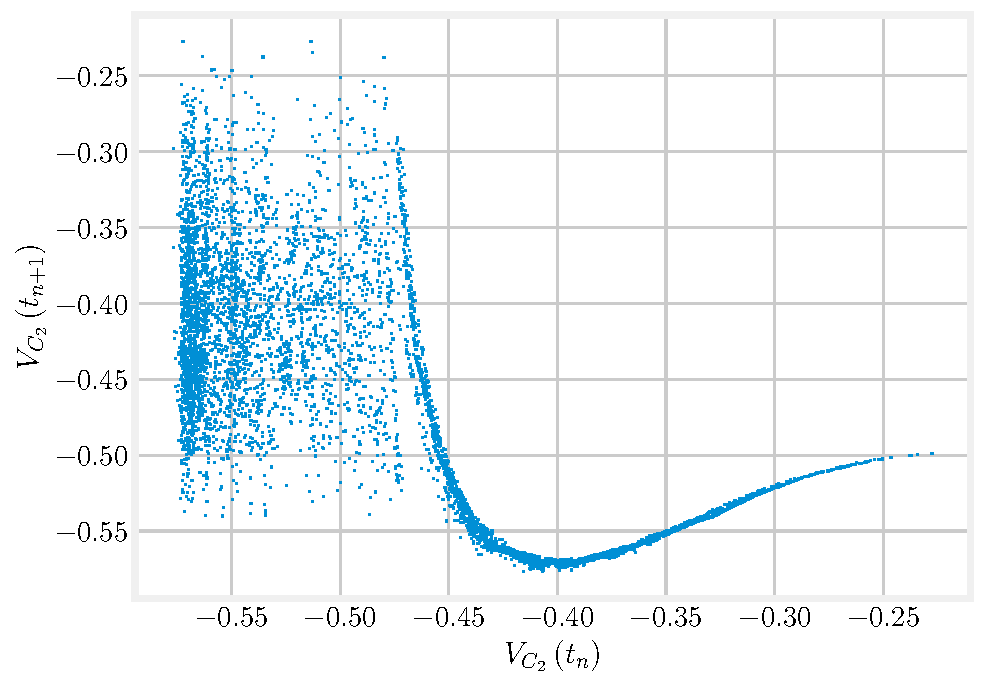
\includegraphics[width=0.44\paperwidth]{V_C_2_t_n_versus_V_C_2_t_n_plus_1}
			\caption{
				Mapa de primer retorno: $V_{C_{2}}\left(t_{n}\right)$ versus $V_{C_{2}}\left(t_{n+1}\right)$.
			}\label{fig:chua_solutions}
		\end{figure}
	\end{minipage}
\end{frame}

\section{Programas}

\begin{frame}[fragile]
	\frametitle{\secname~\parencite[Sección 8.4.2, pág. 246]{Lynch2018}}
	En Python 3.10.6, basados en las bibliotecas NumPy 1.23.1, SciPy 1.9.0 y Matplotlib 3.5.2.
	\begin{minipage}{0.45\textwidth}
		\begin{listing}[H]
			\inputminted[
				fontsize=\tiny,
				highlightlines={13-22,33},
				firstline=13,
				lastline=33,
				escapeinside=||,
				breaklines,
			]{python}{chua_double_scroll.py}
			\caption{
				\small\texttt{chua\_double\_scroll.py} usa la función~\href{https://docs.scipy.org/doc/scipy/reference/generated/scipy.integrate.odeint.html}{\mintinline{python}{scipy.integrate.odeint}}.
			}
		\end{listing}
	\end{minipage}
	\begin{minipage}{0.45\textwidth}
		\begin{listing}[H]
			\inputminted[
				fontsize=\tiny,
				highlightlines={46-48,56-63},
				firstline=43,
				lastline=70,
				escapeinside=||,
				breaklines
			]{python}{poincare_chua.py}
			\caption{
				\small\texttt{poincare\_chua.py} usa la función~\href{https://docs.scipy.org/doc/scipy/reference/generated/scipy.integrate.solve_ivp.html}{\mintinline{python}{scipy.integrate.solve_ivp}}.
			}
		\end{listing}
	\end{minipage}
\end{frame}

\section{Conclusiones}

\begin{frame}
	\frametitle{\secname}
	\begin{itemize}
		\item De la Figura~\ref{fig:changing_beta} podemos ver que el
		      sistema de Chua bajo ciertos parámetros $\alpha=10$  y
		      $\beta_{1}=16.4$, $\beta_{2}=16.401$ es un sistemas caótico
		      ya que para parámetros muy cercanos obtenemos soluciones
		      muy diferentes.

		      \

		\item Para ciertos parámetros $\alpha$, $\beta$, $m_{0}$ y $m_{1}$
		      el sistema de Chua exhibe los atractores en forma de
		      espiral, doble espiral, doble gancho, de tipo Lorenz o
		      Rössler~\parencite{271147}.

		      \


		\item De la Figura~\ref{fig:chua_doble_atractor} logramos implementar un programa para poder obtener la sección de Poincaré y hacer las gráficas para hallar el mapa de primer retorno con el objetivo de ver si las órbitas sean estables.

		      % Con la base de este programa podremos analizar otros sistemas caóticos. % Aplicaciones con la encriptación, redes neuronales.

		      \

		\item Además del análisis con la sección de Poincaré, existen otros métodos como la \emph{aplicación del círculo},
		      el \emph{exponente de Lyapunov más grande}, la \emph{dimensión de correlación}.
	\end{itemize}
\end{frame}
